\chapter{Internet Of Things}
\label{chapter:internetofthings} 

\section{Definition}

The term, Internet of Things, was firstly mentioned by Kevin Ashton in once his presentation in 1999 \cite{ashton2009internet}

Semantically, Internet of Things means ``a world-wide network of interconnected objects uniquely addressable, based on standard communication protocols'' \cite{infso2008networked}. 

\section{Things: The Bridge between Real World and Virtual World}

The ``things'' refers to the ``objects'' in the semantical explanation. The ``things'' are heterogeneous objects. The initial idea of the ``things'' started with Radio-Frequency IDentification (RFID) tags by Auto-ID Labs\footnote{http://www.autoidlabs.org}, a world-wide network of academic research laboratory in the field of networked RFID and emerging sensing technologies. Hereafter, other concepts of ``things'' emerged: NFC tags, Wireless Sensor and Actuator Networks (WSANs), Spime and Smart Items.

\subsection{NFC and WSANs}

NFC is a proximity technology that provides contactless communication by using ISO/IEC 14443 and ISO/IEC 18092. NFC tags utilise Reader/Writer mode, one of the modes that a NFC devices should supports \cite{Madlmayr:SecurityandPrivacy}, to store data and interact with users. A typical scenario is that a NFC tag acts as a smart poster, where a user could place a NFC based mobile phone near a smart poster and thus would retrieve further information. e.g. if a smart poster stores movie poster data, it can forward a user to the movie trailer or its home page. Additionally, there are card emulation mode and Peer-to-Peer mode. Card Emulation Mode e.g. turns a mobile phone into a smart card such as a credit or debit card, and the NFC reader cannot distinguish the difference between the mobile phone and smart cards. Thus, with this features, it can implement a new way of payment system called Mobile Payments. NFC Peer-to-Peer (P2P) mode is designed based on the standards ISO 18092, which allows two NFC devices communicate mutually. \cite{Madlmayr:SecurityandPrivacy}

WSANs are composed of large numbers of minimal capacity sensing, computing, and communicating devices and various types of actuators. WSANs constitute an important and exciting new technology with great potential for improving many current applications. It also creates new revolutionary systems in areas such as global-scale environmental monitoring, precision agriculture, home and assisted living medical care, smart buildings and cities, industrial automation, and numerous military applications. \cite{stankovic2008sensor} 

They are, together with RFID, are recognised as the atomic components that links the real world with the digital world.\cite{sterling2005shaping}

\subsection{Spime and Smart Items}

Spime and Smart Items are also considered to be ``Things'' Oriented Object. Spime is a neologism and firstly mentioned by Bruce Sterling, a science fiction writer, in 2005. Sterling stated that there will be a new kind of object - user-alterable, baroquely multi-featured and programmable - in the future, for which Sterling invented the term ``Spime''. \cite{sterling2005shaping}. Sterling described that the Spime is one of the objects in Internet of Things since Spime enables a thing to be searchable. i.e. A thing can be searched by a search engine from a virtual world to a physical world. \cite{sterling2005shaping} 

Spime is a bit theoretical, but we can find some of its prototype in the real world, and we call them Smart Items \cite{atzori2010internet}.

IoT is also derivative from the vision of ``Internet''. Vasseur and Adam described Smart Objects in their book, Interconnecting Smart Objects with IP: The Next Internet \cite{vasseur2010interconnecting}. A Smart Object is an item equipped with a form of sensor or actuator, a tiny microprocessor, a communication device and a power source. The sensor or actuator gives the smart object the ability to interact with the physical world. Smart Objects are interconnected using the Internet Protocol (IP). 

According to IPSO Alliance, the IP stack is a light protocol that already connects a huge amount of communicating devices and runs on tiny and battery operated embedded devices. This guarantees that IP has all the qualities to make IoT a reality. \cite{atzori2010internet}

\section{Sensors and Actuators}
A sensor detects or measures the physical environment (such as temperature, speed, and location etc) and converts it to a form (such as a digital form) which can be read by human or used for other purpose. For example, a light sensor senses the brightness of the environment, then the sensor converts the brightness into a digital form (data). The data can be, further, transferred to other receivers.

Sensors can interconnect wirelessly, and form a network, which is called wireless sensor network (WSN). WSN monitors the environment or other physical data distributively. According to \cite{culler2004guest}, WSN can be apply to a wide range of uses: monitoring space, things, and the encompassing space. Particularly, the first category, space, which is related to the thesis, covers light, temperature, humidity and other environment data. 

Sensors perform tasks more than measuring environments. The second category applies on things or objects. Sensors, that being the case, are applied more in area of such as, the detection of structures breakages \cite{christin2009wireless}. However, things and the environment are sometimes interconnected and interactive. This is the third category when sensors are used to e.g. monitor the wildlife habitats \cite{culler2004guest} and the interaction between traffic queuing and the frequency of traffic lights switching. In short, the WSN provides a good source of data for Internet of Things.

Sensors collect and transfer data for further use, but an actuator provides controlling functions to a system. e.g. a light switch can turn on and turn off a light; Here the light switch is an actuator. Sensors and Actuators work mutually can optimise processes. For example, sensors are installed in chemical production to bring much greater granularity to monitoring, where the sensor collects data and transfers them to computers which subsequently analyse the data and signal actuators to adjust the processes, such as ingredient mixtures, temperatures, or pressures \cite{chui2010internet}. The whole process can then be automated. 

\section{Internet-based Communication Protocols and Standards}

\subsection{TCP, UDP and IP}
Transmission Control Protocol (TCP), one of the two major transport-layer protocols, provides a reliable bi-directional communication \cite{comer2008computer}. TCP addresses the communication problem between applications with the following major features: 

\begin{itemize}
% You can use this command to set the items in the list closer to each other
% (ITEM SEParation, the vertical space between the list items) 
\setlength{\itemsep}{0pt}
\item Transferring Data over a connection 
\item Connecting two endpoints
\item Data is received the same as it is delivered
\item Data is sent in sequence
\item Reliable startup and shutdown
\end{itemize}

User Datagram Protocol (UDP) is the other major transport-layer protocol used in the Internet \cite{comer2008computer}. Compared with TCP, UDP is less complex and thus less reliable. For example, UDP is connectionless, meaning a message can be sent between two endpoints without prior arrangement; UDP sends and receives individual messages, meaning it does not divide a message into multiple parts.

Internet Protocol (IP) provides a communication mechanism for computers or devices \cite{postel1981internet}. IP distinguishes each computer or device in network by a unique 32-bits number known as Internet Protocol Address (IP address). TCP or UDP packets are usually encapsulated into IP packets.

\subsection{HTTP}

Hypertext Transfer Protocol (HTTP) is an application layer protocol exchanging or transferring contents, such as hypertext, in request/response pattern \cite{fielding1999hypertext}. HTTP is assigned to port number 80 over either TCP or UDP connection \cite{reynolds1994assigned}. HTTP communication, however, usually is established over TCP/IP connections with the default port TCP 80. HTTP can be also established other protocol, such as unreliable UDP.

When a browser requests resources from a server, usually the browser sends a HTTP request to the server. Then the server answers with an HTTP response. Before HTTP 1.1, a pair of request/response is, usually, sent in a single TCP connection. Generally, a TCP connection is expensive to create, while most HTTP 1.0 or older connections use TCP at least efficiency, which leads to congestion and unwanted overhead \cite{spero1994analysis}.  To improve this, HTTP provides connection reuse mechanism \cite{fieldingrfc} by using Keep-Alive in general headers. This mechanism has been further improved in HTTP 1.1, and thus all connections are set to persistency by default. This mechanism aims for reducing CPU and memory usage, pipelining, reducing network congestion, reducing latency the frequency of TCP opening handshakes and error reported improvement. With pipelining, the performance of HTTP 1.1 can be largely improved compared with HTTP 1.0. \cite{nielsen1997network}. 

At this point, HTTP persistent connections seem to be perfect and the WebSocket protocol is unnecessary. The HTTP persistent connection, however, is restricted by its practical consideration. Firstly, Servers are, usually, maintained by setting time-out value. Consequently, the mechanism kills idle connections. e.g. Apache 2.0 server will set the timeout at 15 seconds by default \footnote{http://httpd.apache.org/docs/2.0/mod/core.html\#keepalivetimeout}, while Apache 2.2 reduces the amount down to 5 seconds\footnote{http://httpd.apache.org/docs/2.2/mod/core.html\#keepalivetimeout}. Additionally, this implies that both clients and servers need to be capable to recover from any closed events and subsequently indicates delay in communication. Secondly, any client that use persistent connections is instructed to limit the number of simultaneous connections that they maintain to a given server at the maximum of two, for the purpose of improving HTTP response time and avoiding congestion. 

For a browser, in order to synchronise the information with a web server, normally, there are polling or long-polling over Ajax. When we use Ajax, we retrieve data from a remote server by sending an HTTP Request; and if we would like to retrieve more data, we need to send other HTTP Requests. HTTP request/response will, finally, confront with the fact that it increases the frequency of requesting the web server, with repeatedly connections and disconnections; or increases the workload of the web server to keep the requests open. The problem becomes severe when it happens in the scenario of Internet of Things (IoT) with a large amount of devices interconnected. Figure \ref{fig:client-server-http} illustrates sequence diagram where a client (browser) fetches data from a server using HTTP.

\begin{figure}[ht]
  \begin{center}
    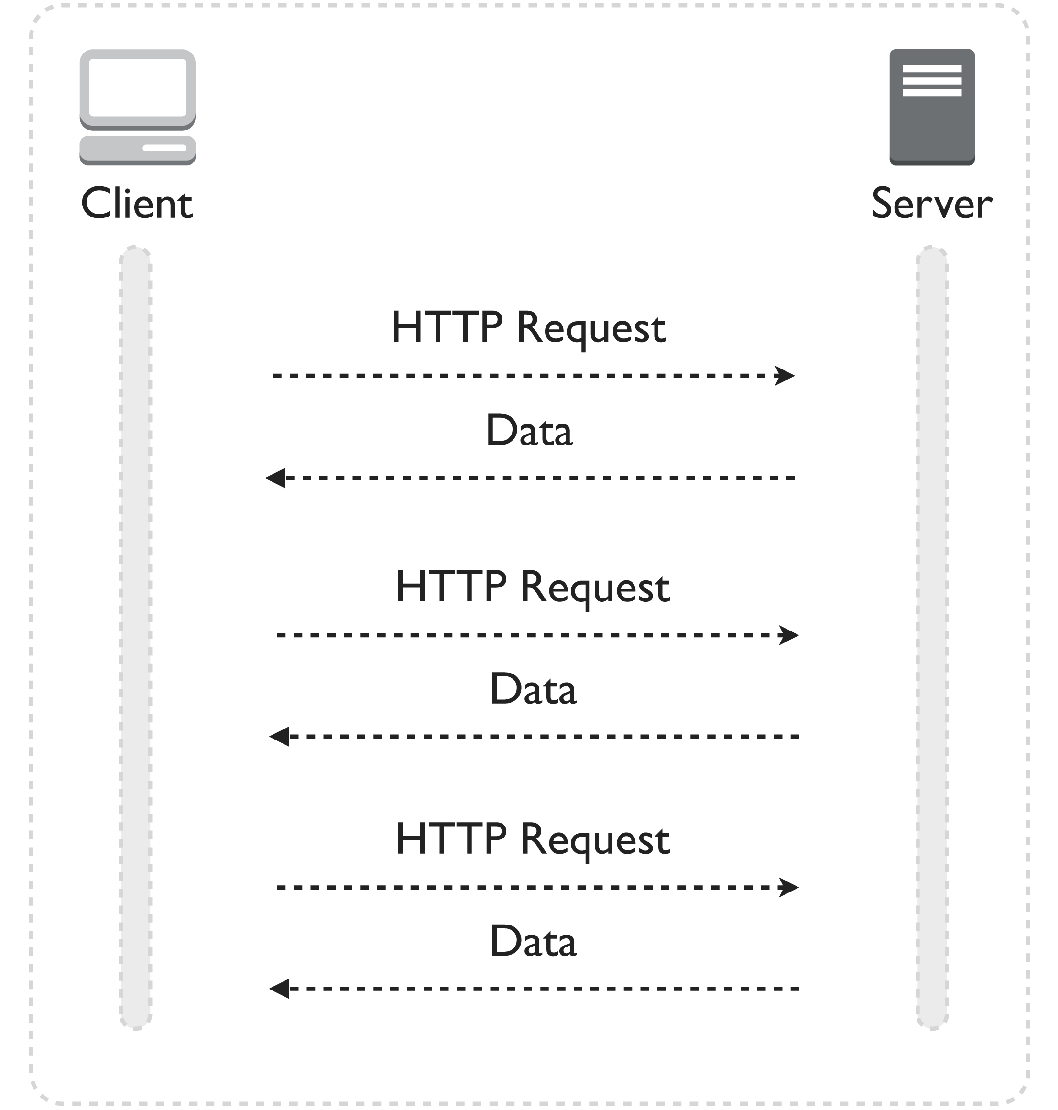
\includegraphics[width=1\textwidth]{images/client-server-http.pdf}
    \caption{A Client Fetches Data from A Server with HTTP}
    \label{fig:client-server-http}
  \end{center}
\end{figure}


However, this approach can radically improved by removing the redundant HTTP Requests. Then we transfer all data over a single TCP connection. This is what we called the WebSocket Protocol. We will expand more about the WebSocket Protocol in Subsection \ref{HTML5andWebSockets}.

\subsection{HTML5 and WebSockets}
\label{HTML5andWebSockets}

HTML5 is hypernym that consist of a large number of web technology \cite{wang2012definitive}. HTML5 covers the following area: new semantics, new CSS styling, multimedia, Graphics \& 3D, Device Access, Performance, offline \& storage and connectivity. Amount all, the connectivity consists of communication technology such as Web Real-Time Communications (WebRTC), Server-Sent Events (SSE), Cross-Document messaging and WebSocket. WebRTC\footnote{http://www.webrtc.org/reference/architecture} provides realtime multimedia communication on web without requiring plugins; SSE provides an API for a browser to receive pushing notification from a server via an HTTP connection \cite{hickson2009server}; While Cross-Document messaging or Web Messaging largely expands the possibility and capability of communication of web browsers with least side-effect on security and privacy. Cross-Document messaging is designed to overcome the same-origin policy.

The goal of WebSocket technology is to provide a mechanism for browser-based applications that need two-way communication with servers that does not rely on opening multiple HTTP connections (e.g. using XMLHttpRequest or <iframe>s and long polling) \footnote{http://www.websocket.org}. Older web technology, like HTTP, remains inefficiencies problems \cite{wang2012definitive}. Firstly, it is not natively designed for nowadays Web Applications with rich contents and interactive demands; Secondly, overheads and unnecessary information cumulate swiftly as the interaction between the client and server continues. WebSocket improves communication problems by solving the above problems, while keeping simplicity. Both WebRTC and WebSocket are in effort to enhance the real-time communication. WebRTC provides APIs that allow web browsers communicate with each other directly, while WebSocket provides the real-time communication mechanism between a client and a server. Figure \ref{fig:client-server-ws} illustrates sequence diagram where a client (browser) fetches data from a server using WebSockets.

\begin{figure}[ht]
  \begin{center}
    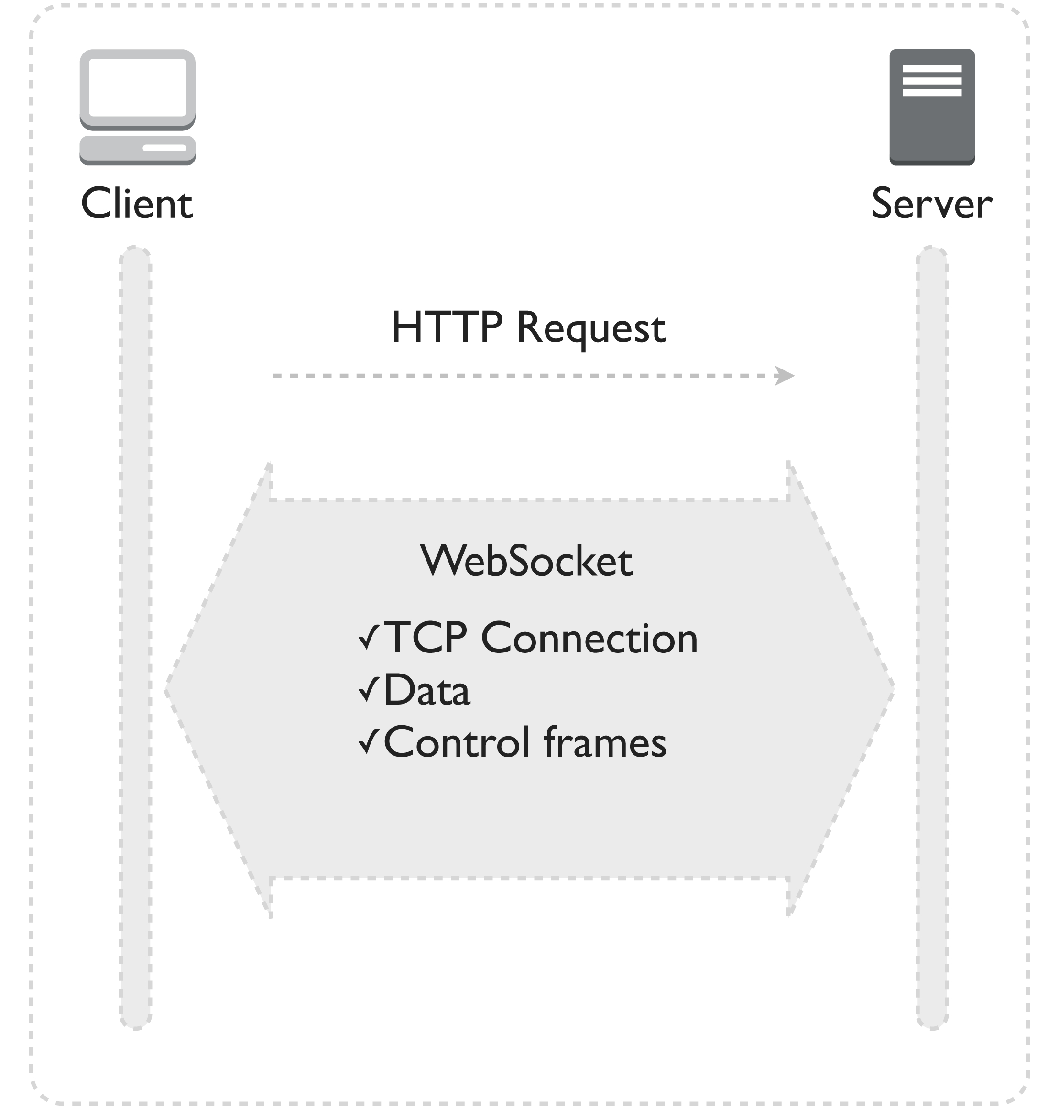
\includegraphics[width=1\textwidth]{images/client-server-ws.pdf}
    \caption{A Client Fetches Data from A Server with WebSockets}
    \label{fig:client-server-ws}
  \end{center}
\end{figure}

\subsection{Internet-based Communication Protocols and Standards with IoT}
The currently architecture of IoT consists three layers \cite{wu2010research}. From top to bottom, they are: application layer, network layer and perception layer. The perception layer consists of the unquietly addressable objects. The network layer connects the objects and connects objects to computers. The application layer makes the IoT data meaningful, useful or extensible.

TCP/IP and UDP ensure the objects communicable in IoT. Moreover, they ensure that the objects can be communicated outside the IoT network. Subsequently, the data, e.g. that sensors collected, is utilisable. For example, the data collected by sensors can be transferred to a data centre and can be further analysed. 

Another issue about IP, Internet Protocol Version 4 (IPv4) is the dominant IP protocol in the Internet currently. IPv4, however, has exhausted \cite{smith2011free} and thus could not meet the `unquietly addressable' requirement in IoT. IP Version 6 (IPv6) is its successor. ``IPv6 enables end-to-end communication, in which any IPv6 `smart things' can connect to any other IPv6 devices or system from any place and at any time. It enables the possible extension of the Internet to any device, sensor or actuator, which can become real nodes of the future Internet.'' \cite{vermesan2011internet}. It primarily provides the following features\cite{deering1998internet}: 

\begin{itemize}
% You can use this command to set the items in the list closer to each other
% (ITEM SEParation, the vertical space between the list items) 
\setlength{\itemsep}{0pt}
\item Expanding addressing capabilities to support a greater amount of addressable nodes. 
\item Simplifying header format to reduce the cost of packet handling.
\item Improving support for extensions and options to allow greater flexibility in the future
\item Flowing labelling capability to label packets and thus to handle, e.g., real-time services.
\item Authentication and privacy capabilities
\end{itemize}

HTTP and WebSocket ensure that IoT can be used or extended by applications. For example, a web interface that can visualise temperature data. Subsequently, IoT network can be directly or indirectly connect to end users. 
